\chapter{Herramientas, técnicas y lenguajes}
\label{chap:herramientas}
	
\section{\textit{Backend}}
\label{sec:herramientas_backend}

Ya que para el \textit{backend} no se necesitaba nada excesivamente complejo, se decidió utilizar el lenguaje de programación Python \cite{python} junto
con el \textit{framework} FastAPI \cite{fastapi}, el cual permite crear APIs REST de forma sencilla. La decisión de utilizar Python, viene también
condicionada por el hecho de que los algoritmos de perfilado de autor utilizados, así como también la mayor parte de los algoritmos de aprendizaje automático, 
están ya programados en Python, evitando así crear nuevos \textit{endpoints}, \textit{sockets} o \textit{bindings} para la ejecución de dichos algoritmos.
Destacar también que el desarrollo ágil en Python favorecía mucho al trabajo debido a su tipado dinámico, a su ejecución interpretada y a su sintaxis sencilla.

\bigskip
Por otro lado, para que el cógido estuviese bien organizado, se decidió utilizar el patrón de diseño DDD (del inglés \textit{Domain-Driven Design}) \cite{ddd}, el cual
permite separar el código en tres capas: la capa de aplicación, la capa de dominio y la capa de infraestructura. La capa de aplicación es la encargada de gestionar
la entrada y salida de la aplicación que, en nuestro caso, es el controlador que maneja los \textit{endpoints} REST; la capa de dominio es la que contiene la lógica
de negocio y las entidades; y la capa de infraestructura es la responsable de administrar las interacciones internas de la aplicación que, en nuestro
caso, se encarga de la comunicación con la base de datos.

\bigskip
Esta es una figura adaptada de https://www.baeldung.com/hexagonal-architecture-ddd-spring Łukasz Ryś 2022
\begin{figure}[H]
	\centering
	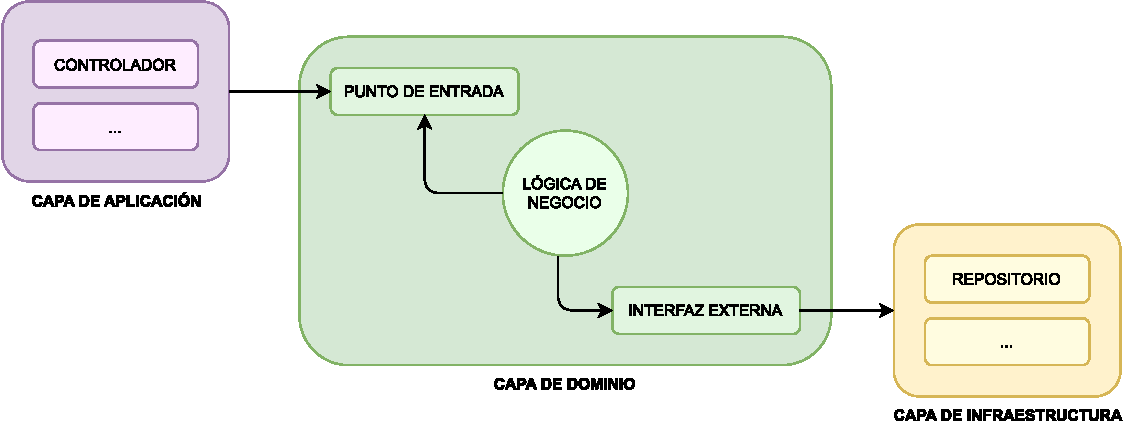
\includegraphics[width=0.9\textwidth]{diagramas/ddd.pdf}
	\caption{Diagrama de capas del patrón de diseño DDD}
	\label{fig:ddd}
\end{figure}

\section{\textit{Frontend}}
\label{sec:herramientas_frontend}

En cuanto al \textit{frontend}, se decidió utilizar NextJS \cite{nextjs} como herramienta para el desarrollo de la interfaz de usuario, dado que ya
se contaba con bastante experiencia previa en su uso. NextJS es un \textit{framework} basado en React \cite{react}, es decir, en la construcción de interfaces dinámicas e interactivas mediante la composición
de elementos que pueden tener estado. Además, este \textit{framework} implementa varias mejoras sobre React como por ejemplo el \textit{server-side rendering}, algo que ayuda en gran medida
al SEO (del inglés \textit{Search Engine Optimizations}), esto es, a que los motores de búsqueda como Google puedan indexar mejor la página y, por tanto, que esta aparezca en una posición superior en los resultados de búsqueda.
Además, también cuenta con optimizaciones para la carga y el renderizado de imágenes o fuentes entre otras.

\bigskip
Todo ello se desarrolló utilizando TypeScript \cite{typescript}, un lenguaje de programación que añade tipado estático a JavaScript
y que está ganando mucha popularidad con respecto a la mentinibilidad, compresión y escalabilidad que proporciona a los proyectos en los que se usa (Stack Overflow, 2023) \cite{stackoverflow2023}.
A mayores, para garantizar la consistencia de todas las entidades, y más en específico de los DTOs (del inglés \textit{Data Transfer Object}), se utilizó Zod \cite{zod}, una librería que permite
definir esquemas de validación de datos, incluyendo el tipo específico de cada campo.

\bigskip
En cuanto el estilado de la página, se optó por emplear SASS (del inglés \textit{Syntactically Awesome Style Sheets}) \cite{sass}, un preprocesador de CSS (del inglés \textit{Cascading Style Sheets}) que añade
funcionalidades extra como son el uso de variables, bucles o anidamiento de clases. Además, dado que se estaba desarrollando
una aplicación novedosa, se buscó crear un estilo propio haciendo uso de CSS "nativo", desmarcándose así de librerías que proporcionasen estilos predefinidos como Bootstrap \cite{bootstrap} o componentes ya implementados
como Material UI \cite{materialui} o Chakra UI \cite{chakraui}. Por otra parte, para la creación de gráficos se utilizó la librería ChartJS \cite{chartjs}, una de las más conocidas
y con más soporte en la actualidad. Finalmente, para implementar las animaciones en la interfaz, se hizo uso, en conjunto con las transiciones nativas
de CSS, de Framer Motion \cite{framermotion}, una librería que permite crear animaciones de una mayor complejidad desde JavaScript/TypeScript. 

\section{Algoritmos de perfilado}
\label{sec:herramientas_algoritmos}

A pesar de que los algoritmos de perfilado se ejecutan en el \textit{backend}, se ha decidido incluirlos en esta sección debido a que se trata de una parte
importante y característica en el proyecto. Decir también que en este caso, las herramientas utilizadas estaban condicinadas, lógicamente,
por aquellas utilizadas en las implementaciones de ambos algoritmos seleccionados.

\bigskip
En cuanto a la parte nuclear del aprendizaje automático, se utlizó Scikit-Learn \cite{scikitlearn}, una librería de Python que proporciona una gran cantidad
de algoritmos pre-implementados, así como también herramientas para la extracción de características o la validación de modelos. Además, se hizo uso
de otras librerías como Tqdm \cite{tqdm}, la cual permite mostrar el progreso de entramiento o predicción de forma visual, Pickle \cite{pickle}, que permite
serializar objetos Python (en nuestro caso los modelos ya entrenados), o NumPy \cite{numpy}, una librería que proporciona estructuras de datos y herramientas para el cálculo científico.

\section{Soporte}
\label{sec:herramientas_soporte}

Para la gestión de tareas, debido a que nuestro ciclo de desarrollo era ágil, se utilizó Trello \cite{trello}, una herramienta que permite crear tableros con listas de tareas, las cuales pueden ser movidas
entre ellas según su estado: pendiente, en progreso o completada. 

\bigskip
Además, debido a la importancia de mantener un control sobre los cambios realizados en el código, se optó por utilizar Git \cite{git} como herramienta de control de versiones junto con GitHub \cite{github}, una plataforma que permite
almacenar repositorios de Git de forma remota, similar a otras como GitLab \cite{gitlab} o BitBucket \cite{bitbucket}.

\bigskip
En cuanto al entorno de desarrollo o IDE (del inglés \textit{Integrated Development Environment}), se utilizó Visual Studio Code \cite{vscode}, un editor gratuito y de código semi-abierto desarrollado por Microsoft, el cual
brinda una gran flexibilidad para trabajar con cualquier lenguaje de programación gracias a sus extensiones. Esto hecho, posibilitó el desarrollo
del \textit{backend}, del \textit{frontend} e inluso de esta memoria en un mismo programa, simplificando la tarea de aprender las peculiaridades de
otros IDEs más específicos. Más en concreto, se utilizaron extensiones como Prettier \cite{prettier} o Black \cite{blackformatter}, las cuales permiten formatear el código de forma automática para JavaScript o Python, respectivamente;
ESLint \cite{eslint}, una herramienta que permite detectar errores en el código JavaScript/TypeScript; o GitLens \cite{gitlens}, una extensión que añade funcionalidades extra con respecto
al control de cambios.

\bigskip
Con respecto, a la elaboración de los diagramas y los \textit{wireframes} que aparecen en este trabajo, se utilizó la herramienta Draw.io \cite{drawio}, la cual permite crear todo tipo de diagramas
\textit{online} de forma gratuita, sin la obligación de registrarse y sin la necesidad de instalar ningún programa, puediendo exportarlos en varios formatos, entre ellos SVG.
Junto a esta herramienta, se utilizó también la librería pgfplots \cite{pgfplots} para la creación de las gráficas en el propio \LaTeX.

\bigskip
\textbf{Mencionar Docker e implementarlo}
